\section{Sele\c{c}\~ao e entrega de conte\'udo}
\label{section:selecaoentrega}
Dentro de uma CDN temos que  nos preocupar com a forma como esse conte\'udo vai catalogado, armazenado e distribu\'ido dentro da rede, o que vimos no item \ref{section:protocolos_interacoes}, como tamb\'em temos que nos preocupar como esse conte\'udo vai chegar at\'e o cliente (usu\'ario) da forma mais otimizada poss\'ivel, ou seja, o servidor o qual vai fornecer as informa\c{c}\~oes para ele ser\'a o mais perto ou mais r\'apido. 
 Temos que destacar tamb\'em a import\^ancia da otimiza\c{c}\~ao do fluxo de informa\c{c}\~ao pela rede. Visto que quanto maior o tr\'afico de informa\c{c}\~ao pela rede significa que a informa\c{c}\~ao est\'a mais distante do usu\'ario e tamb\'em que vai ter um custo maior pela troca intensa de informa\c{c}\~ao. 
 Segundo \cite{krishnamurthy2001use}, na tentativa de otimizar o redirecionamentos de URL para o usu\'ario se sacramentou dois tipos de t\'ecnicas de redirecionamentos, Full - site e Partial - site.

\subsection{Full - site}
Na t\'ecnica de Full-site todo o conte\'udo \'e entregado ao usu\'ario de um servidor ponta \'unico. Ou seja, o usu\'ario faz uma requisi\c{c}\~ao ao servidor principal, onde o mesmo processa um algoritmo de roteamento para encontrar o servidor ponta que melhor se enquadra como resposta, e ent\~ao retorna ao usu\'ario o endere\c{c}o onde ent\~ao ser\'a consumido por fim todas as informa\c{c}\~oes requisitadas. 
 \'E importante salientar que essa t\'ecnica \'e amplamente utilizada por servi\c{c}os que fazem pouco uso de dados da rede. Uma p\'agina est\'atica da web, por exemplo, se encaixaria perfeitamente nesse contexto. Visto que possui baixo grau de modifica\c{c}\~oes e seu tamanho \'e pequeno perto de outros tipos de m\'idias que circulam na web.

\subsection{Partial - site}
J\'a redirecionamentos do tipo Partial-sites os servidores principais retornam para o usu\'ario uma parte do conte\'udo e disparam, automaticamente, um algoritmo de roteamento para encontrar o restante da informa\c{c}\~ao e retornar ao usu\'ario. Conforme podemos ver na figura \ref{figura:entrega_conteudo}
\begin{figure}[H]
\caption{Entrega de conte\'udo}
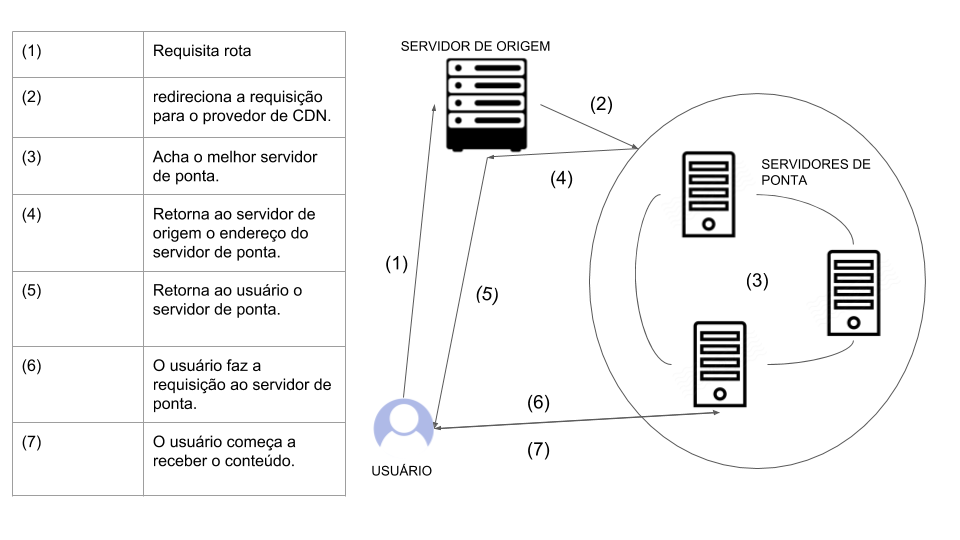
\includegraphics[height=9cm]{Figuras/entrega_conteudo.png} 
\label{figura:entrega_conteudo}
\end{figure}
Nela podemos ver que todo o processo acontece em basicamente sete etapas. (1) o usu\'ario faz uma requisi\c{c}\~ao ao servidor principal onde este dispara (2) um roteamento (3) para buscar qual \'e o melhor servidor para aquele usu\'ario. Depois, em (4) o servidor principal recebe a identifica\c{c}\~ao do servidor de ponta e repassa ao usu\'ario (5) juntamente com um arquivo que cont\'em as informa\c{c}\~oes centrais que normalmente s\~ao iguais para o mundo todo. Em seguida o usu\'ario come\c{c}a a enviar (6) e receber (7) informa\c{c}\~oes com o servidor de ponta.

 Entretanto h\'a em (3) diversas formas de fazer esse roteamento quanto a distribui\c{c}\~ao do conte\'udo pela rede e quanto a aglomera\c{c}\~ao desse conte\'udo dentro do servidores de cache. 
 Tipo de distribui\c{c}\~ao nada mais \'e do que a forma como o conte\'udo vai ser disperso na rede, como esse conte\'udo vai se aproximar do n\'o que est\'a mais perto do usu\'ario. 

Os tipos de distribui\c{c}\~ao mais frequentemente utilizados s\~ao o emp\'irico e o por popularidade.

Emp\'irico trata, como o pr\'oprio nome diz, de uma forma de distribui\c{c}\~ao sem nenhum conhecimento espec\'ifico a respeito, utilizando-se apenas um conhecimento experimental de onde seria melhor posicionado o conte\'udo.
 Em um esquema baseado em popularidade a distribui\c{c}\~ao \'e feita conforme a notoriedade. Ou seja, quanto maior o n\'umero de requisi\c{c}\~oes a um conte\'udo, mais ele ser\'a distribu\'ido nos servidores de ponta perto do usu\'ario.
 Ambos esquemas n\~ao s\~ao necessariamente excludentes, pode-se inicialmente aplicar a forma empir\'ica para gerar dados a respeito da distribui\c{c}\~ao e depois utilizar esses dados para aplicar o modo de popularidade.
	
Tamb\'em existe as formas de aglomera\c{c}\~oes de conte\'udo. Isso existe porque os conte\'udos podem ser conjuntos de objetos ou objetos independentes. 
As formas de aglomera\c{c}\~oes s\~ao por objeto e por conjunto de objetos.

Aglomera\c{c}\~ao por objeto vai juntar os objetos mais selecionados e distribu\'i-los individualmente entre os servidores. J\'a por conjunto de objetos ele vai separ\'a-los em grupos e distribui-los em conjuntos. 
 Podemos exemplicar da seguinte forma: Em um site temos v\'arios elementos, temos o HTML, temos o CSS e temos a m\'idia de um v\'ideo qualquer. Podemos separar da seguinte forma: temos 3 elementos onde 2 deles s\~ao altamente dependentes(HTML e CSS) e temos 1 que pode ser diferente em cada regi\~ao do pa\'is, que \'e o v\'ideo. 
 Ent\~ao podemos misturar as formas de aglomera\c{c}\~oes. Para o HTML e para o CSS agrupamos em conjuntos de objetos; e para o v\'ideo fazemos a aglomera\c{c}\~ao por objeto,j\'a que ser\'a distribu\'ido de maneira independente nos servidores.

Analisando os tipos,perceber-se que nenhuma das op\c{c}\~oes s\~ao excludentes entre s\'i, pode-se combinar quaisquer tipo de distribui\c{c}\~ao e aglomera\c{c}\~ao e as escolhas v\~ao depender das necessidades de cada aplica\c{c}\~ao.\'E necess\'ario uma an\'alise minuciosa de cada aplica\c{c}\~ao para chegar em um veredito da melhor abordagem.
\subsection{VOD}
\label{subsec:vod}
\paragraph{VOD - Video on Demand} - Segundo \cite{garfinkle1996video}, \'e um sistema de que proporciona uma interface de comunica\c{c}\~ao com o usu\'ario de produtos dispon\'iveis de uma esta\c{c}\~ao central remota.
 \'E um sistema muito utilizado por operadoras de conte\'udo onde \'e o cliente quem decide o hor\'ario que ir\'a consumir determinado conte\'udo.
 Isso permite \`as pessoas que tinham que esperar o hor\'ario certo para consumir determinado conte\'udo, poderem a qualquer momento e em qualquer lugar fazer uso do mesmo.
\paragraph{Microsoft Smooth Streaming} \'E um sistema de consumo de v\'ideo onde a qualidade do v\'ideo transmitida vai ser definida conforme a qualidade da banda dispon\'ivel. Clientes que possuem alta disponibilidade de banda ter\~ao maior qualidade do v\'ideo. 
 Para conseguir tocar um v\'ideo nesse formato o player do usu\'ario tem que ser capaz de interpretar um manifesto que cont\'em dentro de outras coisas, o caminho de onde est\'a localizado a m\'idia desejada. 
 J\'a para conseguir fazer a transi\c{c}\~ao de qualidade o v\'ideo \'e quebrado em pequenos peda\c{c}os chamados de "chunks". Ent\~ao, conforme \'e verificada um aumento ou decremento da banda dispon\'ivel o player come\c{c}ar que consumir chunks de qualidade diferente da atual alternando assim o \textit{bitrate} do v\'ideo que est\'a sendo consumido. 
 No artigo \cite{zambelli2009iis} podemos ver todas as aplica\c{c}\~oes e implica\c{c}\~oes dessa forma de consumo de m\'idia.
\subsection{VOD na pr\'atica}
\label{subsubsection:vod_exemplo}
Agora vamos ilustrar com um exemplo mais pr\'atico. Utilizaremos uma requisi\c{c}\~ao de uma URL de um VOD (Video On Demand) onde a parte de roteamento \'e feita no usu\'ario. A aplica\c{c}\~ao do usu\'ario faz uma requisi\c{c}\~ao \`a CDN e enquanto o cabe\c{c}alho da resposta n\~ao for 200 ele vai ler um campo dentro do cabe\c{c}alho de resposta e fazer uma nova requisi\c{c}\~ao. A figura  \ref{figura:vod_redirect_exemple} ilustra a situa\c{c}\~ao.

\begin{figure}[H]
\caption{Redirecionamento de CDN}
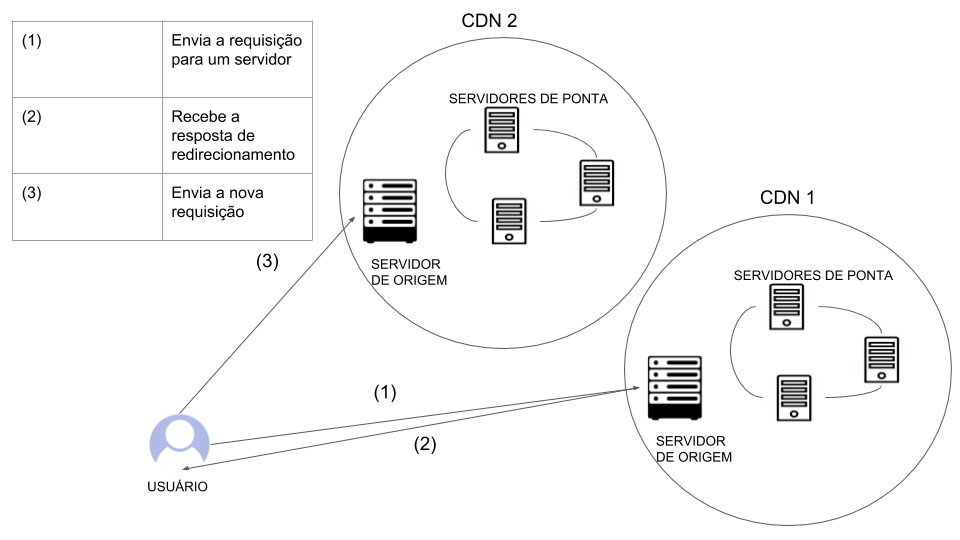
\includegraphics[width=15cm]{Figuras/vod_redirect_exemple.png} 
\label{figura:vod_redirect_exemple}
\end{figure}